\documentclass[11pt]{article}
\usepackage{fullpage}
\usepackage{graphicx}
\usepackage{amsmath}
\usepackage{amssymb}
\usepackage{amsthm}
\usepackage{algorithm}
\usepackage{algorithmic}
\usepackage{float}
%\setlength{\hoffset}{-1.0cm}
%\setlength{\voffset}{-1.0cm}
%\setlength{\textheight}{8.5in}
%\setlength{\textwidth}{6.0in}

% Some utilities

\graphicspath{ {./images/} }
\newcommand{\comment}[1]{}
\newenvironment{definition}[1][Definition]{\begin{trivlist}
\item[\hskip \labelsep {\bfseries #1}]}{\end{trivlist}}
\newenvironment{remark}[1][Remark]{\begin{trivlist}
\item[\hskip \labelsep {\bfseries #1}]}{\end{trivlist}}
\newtheorem{theorem}{Theorem}[section]
\newtheorem{lemma}[theorem]{Lemma}

\title{ Motion Planning for Baxter Arm }

\author{Sean Vierling, Matthew Robinson, Dr. Chakraborty }
\date{May 17,  2021}
\begin{document}
\maketitle

\section*{Abstract}
The Baxter arm is a 7 Degree of Freedom robotic manipulator that is used in this paper to implement a motion planning algorithm. Upon completion of a Python program that utilized the Iterative Motion Planning Algorithm the Baxter arm is capable of completing a variety of tasks within its joint limits. The task being analyzed for our example will be opening a door knob. The Python script will run through the Iterative Motion Planning Algorithm and create a path for the robot arm to follow. The script saves the joint angles of each link throughout the path of the arm. Additionally, the path of the end effector along with visual representations of the links are plotted upon termination of the script. These figures help to verify a successful completion of a motion planning Python program that could be used to create paths for a variety of tasks for a robotic manipulator up to n-DoF. 

\newpage
\section{Introduction}
Multidegree of freedom robotic manipulators have many uses in modern day. Robotic arms exist both as stand alone stationary robots used for manufacturing or can be integrated with mobile robots. An example of this integration can be seen with the walking robot dog, Spot.  Created by Boston Dynamics, Spot is capable of opening doors, closing pipe valves and fetching tools. The practicable application of robotic manipulators is only expanding and are continuing to be employed by more industries. In order to take advantage of the benefits that a robotic manipulator can offer, proper trajectory planning algorithms must be implemented to ensure successful completions of various tasks. Robotic manipulators come in various packages. Some are made of only revolute joints while others consist of a combination of revolute and prismatic. Additionally, the degrees of freedom of each manipulator can vary greatly. Being able to employ a single program capable of path generation for any robotic manipulator is an integral part in ensuring industries are capable of using robotic arms for their specific needs.  

\section{Problem Statement}
To test the implementation of the motion planning algorithm, the use of a Baxter 7 DoF robotic manipulator will be used to open a door knob. The Baxter arm contains 7 revolute joints linked in a single chain. Eight individual length parameters were defined to accurately define joint axes and joint positions, and are named $\l_1$ through $\l_8$. These eight parameters are not all following a single joint and ending at the next adjacent joint, but rather are defined based on the geometry of the physical links, and are somewhat arbitrary by nature. 
\newline

The Baxter arm will begin in its neutral position. In this position all angles are set to zero. The initial configuration of the end-effector is rotated about the z-axis by -$\frac{\pi}{4}$ as seen in the initial transformation matrix. Mathematically this initial configuration can be seen in the transformation matrix $\ gst_0 $ seen below.

$$
\  gst_0 = \begin{pmatrix}
\frac{1}{\sqrt{2}}&\frac{1}{\sqrt{2}}&0&(\l_2+\l_3+\l_5+\l_8)\cdot cos(\frac{\pi}{4})\\
\frac{-1}{\sqrt{2}}&\frac{1}{\sqrt{2}}&0&(\l_2+\l_3+\l_5+\l_8)\cdot sin(\frac{\pi}{4})\\
0&0&1&\l_1-\l_4-\l_6\\
0&0&0&1\\
\end{pmatrix}
$$
\newline
The manipulator will then move from its initial configuration of $\ gst_0$ to the position of the door knob where it will grasp it by utilizing the end-effector. The initial position of the knob is assumed to be directly in front of the baxter robot along its spatial y-axis. This brings the orientation of the end-effector to be aligned with the spatial orientation. The end-effector is now only translated along the y and z axes relative to the spatial frame. The new configuration of the end-effector is given by the transformation matrix $\ g_{handle}$. 

$$
\  g_{handle} = \begin{pmatrix}
1&0&0&0\\
0&1&0&\l_2+\l_3+\l_5+\l_8 - 300\\
0&0&1&\l_1-\l_4-\l_6\\
0&0&0&1\\
\end{pmatrix}
$$
\newline
After grasping the door handle, the end-effector must maintain the same position while rotating the door handle 90 degrees. The rotation of the door handle will be about the y-axis of the end-effector as seen in the transformation matrix below. This transformation matrix will be defined as $\ g_{twist}$.

$$
\  g_{twist} = \begin{pmatrix}
0&0&-1&0\\
0&1&0&\l_2+\l_3+\l_5+\l_8 - 300\\
1&0&0&\l_1-\l_4-\l_6\\
0&0&0&1\\
\end{pmatrix}
$$
\newline

Lastly, to open the door, the end-effector must maintain the same orientation with respect to the door handle while translating the handle about the axis of the door hinge.  The door will be rotated about the hinge only by 22.5 degrees, or $\frac{\pi}{4}$ radians, as to avoid potential collisions with the door. This final transformation matrix will be defined as $\ g_{open}$.

$$
\  g_{open} = \begin{pmatrix}
0&0&-1&(\l_2 + \l_3 + \l_5+\l_8 - 400)\cdot cos(\frac{3\cdot\pi}{8}))\\
0&1&0&(\l_2 + \l_3 + \l_5+\l_8 - 400)\cdot sin(\frac{3\cdot\pi}{8}))\\
1&0&0&\l_1-\l_4-\l_6\\
0&0&0&1\\
\end{pmatrix}
$$
\newline

The goal of the trajectory planning is not to define the initial and final configurations of each step of the door opening process but define the path in which the end effector will take to get from one configuration to the next. The process needs to be broken down in discrete steps obtaining the angles of each joint throughout the path of the end-effector. 


\section{Solution Approach}
In order to create a path for the robotic manipulator to follow, an iterative motion planning algorithm was employed known as Screw Linear Interpolation, or ScLERP. The ScLERP method takes into account the current pose of the manipulator and the goal pose of the manipulator and iteratively defines a screw vector that approaches the goal pose from the current pose. Using a simple iterative algorithm, you can then break up the path defined by the screw into $\frac{1}{\tau}$ different sections, and linearly interpolate through each of those sections, where $\tau$ is a value between 0 and 1 and will be discussed later in more detail. With each iteration of the interpolation of each segment, the ScLERP method determines the next joint space configuration necessary to continue along the path. The algorithm can be broken down into seven different steps. 
\newline

In order to use ScLERP for any given manipulator, the inputs required to define the specific manipulator are the joint axes defined relative to the spatial frame, or $axis_{joints}$, the position vectors from the spatial frame to each axis, or $q_{joints}$, and the neutral configuration of the manipulator where all joint angles are 0, defines by the initial transformation matrix $gst_0$. These values can be seen below:
\newline

$l_1 = 270.35$, $l_2 = 69$, $l_3 = 364.35$, $l_4 = 69$, $l_5 = 374.29$, $l_6 = 10$, $l_7 = 374.42$, $l_8 = 229.525$
\newline

$axis_{joints} = [[0, 0, 1], [\frac{-1}{\sqrt{2}}, \frac{1}{\sqrt{2}}, 0], [\frac{1}{\sqrt{2}}, \frac{1}{\sqrt{2}}, 0], [\frac{-1}{\sqrt{2}}, \frac{1}{\sqrt{2}}, 0], [\frac{1}{\sqrt{2}}, \frac{1}{\sqrt{2}}, 0], [\frac{-1}{\sqrt{2}}, \frac{1}{\sqrt{2}}, 0], [\frac{1}{\sqrt{2}}, \frac{1}{\sqrt{2}}, 0]]$
\newline

$q_{joints} = [[0, 0, 0], [l2 \cdot cos(\frac{\pi}{4}), l2 \cdot sin(\frac{\pi}{4}), l1], [0, 0, l1], [(l2 + l3) \cdot cos(\frac{\pi}{4}), (l2 + l3) \cdot sin(\frac{\pi}{4}), l1 - l4], [(l2 + l3) \cdot cos(\frac{\pi}{4}), (l2 + l3) \cdot sin(\frac{\pi}{4}), l1 - l4], [(l2 + l3 + l5) \cdot cos(\frac{\pi}{4}), (l2 + l3 + l5) \cdot sin(\frac{\pi}{4}), l1 - l4 - l6], [(l2 + l3 + l5) \cdot cos(\frac{\pi}{4}), (l2 + l3 + l5) \cdot sin(\frac{\pi}{4}), l1 - l4 - l6]]$
\newline

 Furthermore, the input requirements for ScLERP to define a path are the starting configuration of the end-effector using a transformation matrix and the corresponding starting joint space configuration, defined as $g$(0) and $\Theta$(0) respectively, as well as the final transformation matrix  $g_{final}$. 
\newline

The first initial step to this process, which can be referred to as step 0, is to convert the final transformation matrix $g_{final}$ to a unit dual quaternion $A_f$. Next, the first real iterative step is to convert the current transformation matrix into a unit dual quaternion A(t) and a concatenation of the position and rotation unit quaternion denoted by $\gamma$(t). Step two utilizes the unit dual quaternions that define the current and final configuration and determines what the next pose should be along the screw path. Mathematically step two can be written as A(t+1) = A(t)  $\otimes$  (A*(t) $\otimes$ $\ A_f$)$^\tau$. 
\newline

Here, $\tau$ denotes the step size desired between the current and final positions, and again, is a value between 0 and 1. A common issue with this iterative method is caused by a constant small $\tau$ value. When $\tau$ is small and static, as the current pose approaches the goal pose, the step size approaches 0 and the current pose continues to approach the goal pose at a decreasing rate. To solve this, first, the remaining screw distance is calcualted each iteration, calculated as A*(t) $\otimes$ $\ A_f$. From this unit dual quaternion, the remaining rotation angle $\theta_{remaining}$ and translation distance $p_{remaining}$ can be determined and compared to the initial rotation angle, $\theta_i$, and translation distance,  $p_i$. These values are then normalized by dividing the rotation angle or displacement remaining from the current pose by the rotation angle or displacement remaining from the initial pose, or $\Delta \theta = \frac{\theta_{remaining}}{\theta_i}$ and $\Delta p = \frac{p_{remaining}}{p_i}$. These normalized differences should remain less than 1 and in fact approach 0 as the current pose approaches the goal pose. A total difference value is then defined as $d = \frac{(\Delta \theta + \Delta p)}{2}$, and $\tau$ is then increased each iteration by $\frac{0.001}{d}$. While this method is somewhat arbitrary, it greatly reduces the necessary iterations for any given trajectory planning.
\newline

Step three utilizes the next desired pose in the interpolation process, defined as a unit dual quaternion in step two, and transforms it into a 7x1 concatenated vector known as $\gamma$(t+1). Within step four the angles of each link are computed by using the time-discretized velocity kinematics equations. Mathematically this can be written as $\Theta$(t+1) = $\Theta$(t) + B($\Theta$(t))($\gamma$(t+1)-$\gamma$(t)). Here, $B$ is a jacobian-like matrix that is a function of the joint configuration of the manipulator, and relates $d \gamma$ to $d \theta$, the change in the joint velocties. Using the values from $\Theta$(t+1), the forward kinematics of the manipulator can be computed resulting in the next pose which can be written as a transformation matrix $\bar{g}$(t+1). Step six checks if $\bar{g}$(t+1) is close to $\ g_{final}$. If $\bar{g}$(t+1) is close enough to  $ \ g_{final}$ the position is reached and the algorithm ends. However, if  $\bar{g}$(t+1) is not close enough step seven is implemented. Within step seven, $\bar{g}$(t+1) become the new g(t+1) and $\Theta$(t+1) becomes the new $\Theta$(t). The process then begins at step one again.
\newline

The iterative motion planning algorithm was programmed using two different classes. The first class is a quaternion math class that contains methods for the various math functions needed for quaternions. This class is named Quat Math. The second class, Motion Planner, is a hereditary of the first class, and consists of methods for computing sub-parts of each step of the iterative process. A single method in the Motion Planner class, iteration, was used, which calculated one iteration of the entire motion planning algorithm up to the next set of theta values. A second method was then used to update any necessary values, including $\tau$, for the next iteration. To use this class for this method, each different specified path needed was defined as a motion planning object. For instance, the first path required, which was moving from the neutral position to the handle of the door, was defined as a motion planner object, with input parameters defining the initial and final position and orientation of the end-effector. Then, using a while loop, the iteration and update methods were repeatedly called for that object until the actual position and orientation of the end effector was within a desired error. Additionally, in order to ensure that the configuration was obtainable, joint angle ranges were set for each joint of the Baxter arm. While running through the iteration, the angles of each joint were checked in each configuration to ensure they remained within their limitations.      

\section{Results}
The ScLERP method seemed to allow for high precision motion planning, and with the iterative increase in $\tau$, it took close to minimal iterations. The matplotlib library on Python was used to map not only the path of the end effector, but to display the initial and final orientation of the baxter robot for each move.

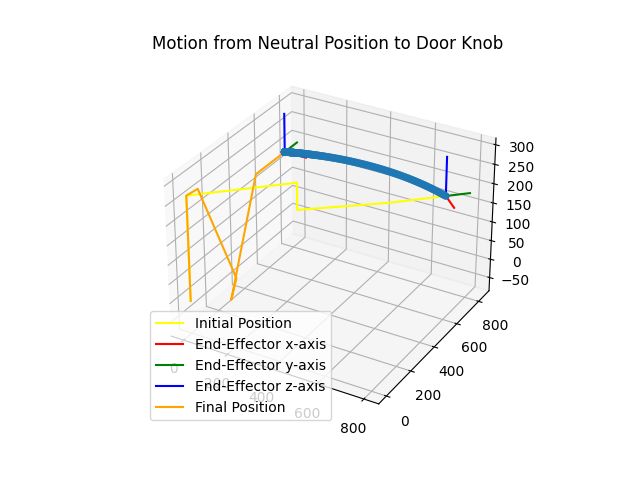
\includegraphics{Motion from Neutral Position to Door Knob}
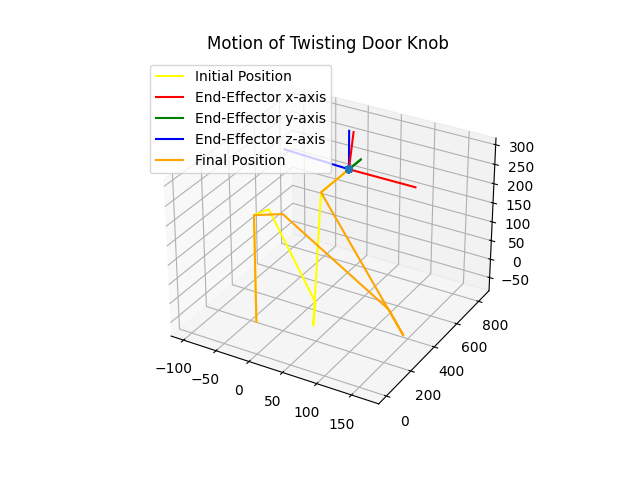
\includegraphics{Motion of Twisting Door Knob}
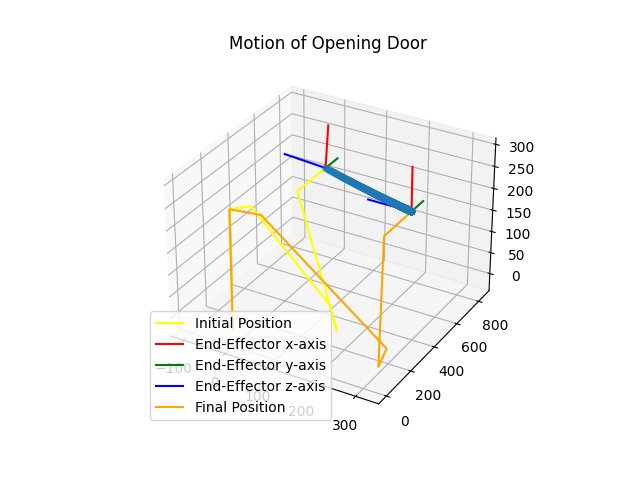
\includegraphics{Motion of Opening Door}

\section{Conclusion}
The final outcome of implementing the Iterative Motion Planning algorithm into a Python script yielded a successful way to generate paths for robotic manipulators with n-degrees of freedom. The script is capable of displaying the configuration of the robot in each pose as well as the path taken by the end-effector in Euclidean space. Though the main goal of path generation is achieved, the program could be expanded to enhance the path taken by the manipulator. The first enhancement could be made by implementing obstacle avoidance with the Python program. This would allow the program to be used in more realistic scenarios where the object being interacted with is not isolated from the real world. The second enhancement could be made to the check thetas method. This method checks to make sure all joint angles lie within their limits while the manipulator moves along the path. An improvement could be made to this method by allowing the method to generate a new path that satisfies those joint limits rather than just displaying an error method. Overall, this program yields a robust starting point for various different implementations of path generation.   

\end{document}
